\documentclass[11pt,american,czech]{article}
\usepackage[a4paper]{geometry}
\geometry{verbose,tmargin=2cm,bmargin=2cm,lmargin=2cm,rmargin=2cm,headheight=0.8cm,headsep=1cm,footskip=0.5cm}
\setcounter{secnumdepth}{3}
\usepackage{url}
\usepackage{amsmath}
\usepackage{amsthm}
\usepackage{amssymb}
\usepackage{graphicx}
\usepackage{setspace}
\usepackage{enumerate} %roman enumiration
\usepackage{threeparttable}
\usepackage{algorithmic}
\usepackage{algorithm}
\usepackage{subfigure}
\usepackage[width=.75\textwidth]{caption}
\usepackage{array}
\usepackage[utf8]{inputenc} % Required for inputting international characters
\usepackage[T1]{fontenc} % Output font encoding for international characters
\usepackage{mathpazo} % Palatino font


\pagenumbering{arabic}

\makeatletter
%%%%%%%%%%%%%%%%%%%%%%%%%%%%%% Algorithms
% Define a \HEADER{Title} ... \ENDHEADER block
\newcommand{\HEADER}[1]{\ALC@it\underline{\textsc{#1}}\begin{ALC@g}}
	\newcommand{\ENDHEADER}{\end{ALC@g}}
\renewcommand*{\ALG@name}{Algoritmus}
\algsetup{indent=2em} 
\renewcommand{\algorithmiccomment}[1]{\hspace{2em}// #1} 
\makeatother

%% Use Times New Roman font for text and Belleek font for math
%% Please make sure that the 'esint' package is turned off in the
%% 'Math options' page.
\usepackage[varg]{txfonts}


%% Indent even the first paragraph in each section
\usepackage{indentfirst}

% completely avoid orphans (first lines of a new paragraph on the bottom of a page)
\clubpenalty=9500

% completely avoid widows (last lines of paragraph on a new page)
\widowpenalty=9500

% disable hyphenation of acronyms
\hyphenation{CDFA HARDI HiPPIES IKEM InterTrack MEGIDDO MIMD MPFA DICOM ASCLEPIOS MedInria}

%%---------------------------------------------------------------------

%% Print out all vectors in bold type instead of printing an arrow above them
%%\renewcommand{\vec}[1]{\boldsymbol{#1}}

% Replace standard \cite by the parenthetical variant \citep
%\renewcommand{\cite}{\citep}

\makeatother
%\pagestyle{empty} %turns off page numbering
\usepackage{babel}
\newcommand*\Laplace{\mathop{}\!\mathbin\bigtriangleup}
\newcommand*\midpoint[1]{\overline{#1}}

\begin{document}
\selectlanguage{czech}
\def\documentdate{...}


\begin{titlepage} % Suppresses displaying the page number on the title page and the subsequent page counts as page 1
	\newcommand{\HRule}{\rule{\linewidth}{0.5mm}} % Defines a new command for horizontal lines, change thickness here
	\center % Centre everything on the page	
	
	\textsc{\LARGE FJFI ČVUT}\\[1.5cm] % Main heading such as the name of your university/college
	\vfill
%	
\includegraphics[width=0.2\textwidth]{Images/TITLE/fjfi}\\[1cm] % Include a department/university logo - this will require the graphicx package	
	
%	\noindent %
%	\begin{minipage}[c]{3cm}%
%		\noindent \begin{center}
%			
\includegraphics[width=3cm,height=3cm,keepaspectratio]{Images/TITLE/cvut}
%			\par\end{center}%
%	\end{minipage}%
%	\begin{minipage}[c]{0.6\linewidth}%
%		\begin{center}
%			\textsc{\large{}České vysoké učení technické v Praze}{\large{}}\\
%			{\large{}Fakulta jaderná a fyzikálně inženýrská}
%			\par\end{center}%
%	\end{minipage}%
%	\begin{minipage}[c]{3cm}%
%		\noindent \begin{center}
%		
\includegraphics[width=3cm,height=3cm,keepaspectratio]{Images/TITLE/fjfi}
%		\par\end{center}%
%	\end{minipage}
%	\vspace{3cm}
	
	\textsc{\Large aplikace statistických metod}\\[0.5cm] % Major heading such as course name
	\textsc{\large soubor č. 6}\\[0.5cm] % Minor heading such as course title
	\HRule\\[0.4cm]
	{\huge\bfseries Protokol analýzy dat}\\[0.4cm] % Title of your document
	\HRule\\[1.5cm]
	{\large\textit{Autor:}}\\
	Vladislav \textsc{Belov}\\
	\vfill\vfill\vfill\vfill\vfill\vfill\vfill % Position the date 3/4 down the remaining page
	{\large\today} % Date, change the \today to a set date if you want to be precise
	
	%------------------------------------------------
	%	Logo
	%------------------------------------------------
	
%	\vfill\vfill
%	
\includegraphics[width=0.2\textwidth]{Images/TITLE/fjfi}\\[1cm] % Include a department/university logo - this will require the graphicx package
%	
	%----------------------------------------------------------------------------------------
	
	\vfill % Push the date up 1/4 of the remaining page
	
\end{titlepage}

%\tableofcontents
%\newpage{}

\section{Úvod}\label{sec:1}

V rámci této práce je provedena analýza datového souboru "Fitting Percentage of Body Fat to Simple Body Measurements", kde jsou představeny měření váhy, výšky, obvodů různých částí těla a také je vyčísleno procento tuku pro $252$ mužů.

\section{Deskriptivní statistika}

\subsection{Numerická analýza}

V první části této práce vybereme několik základních měření poskytující obecný přehled o populaci. V Tab.~\ref{tab:desc1}-\ref{tab:desc2} lze nalézt deskriptivní statistiky takových parametrů jako váha, výška a věk.

\medskip

\begin{table}[ht!]
	\centering
	\begin{tabular}{|c||c|c|c|c|c|c|}
		\hline 
		Proměnná &  Min. hodnota &  1. kvantil &  Medián &  Střední hodnota &  3. kvantil & Max. hodnota   \\ 
		\hline \hline 
		Celková váha & 118.5 & 159 & 176.5 & 178.9 & 197 & 363.1   \\ 
		\hline 
		Váha bez tuku & 105.9 & 131.3 & 141.6 & 143.7 & 153.9 & 240.5   \\ 
		\hline 
		Výška & 29.5 & 68.25 & 70 & 70.15 & 72.25 & 77.75   \\ 
		\hline 
	\end{tabular} 
	\caption{Numerická deskriptivní statistika pro váhu a výšku populace. Váha je měřena v librách, výška v palcích.}	
	\label{tab:desc1}
\end{table}

\begin{table}[ht!]
	\centering
	\begin{tabular}{|c||c|c|}
		\hline 
		Věk &  Počet zástupců &  \%   \\ 
		\hline \hline 
		22-34 & 53 & 21.03   \\
		\hline
		35-49 & 116 & 46.03  \\
		\hline  
		50-64 & 62 &  24.6  \\
		\hline 
		65-81 & 21 &  8.34  \\
		\hline 
	
	\end{tabular} 
	\caption{Numerická deskriptivní statistika pro věk.}
	\label{tab:desc2}	
\end{table}
 
\subsection{Grafická analýza}

\newpage

\begin{figure}[ht!]
	\centering
	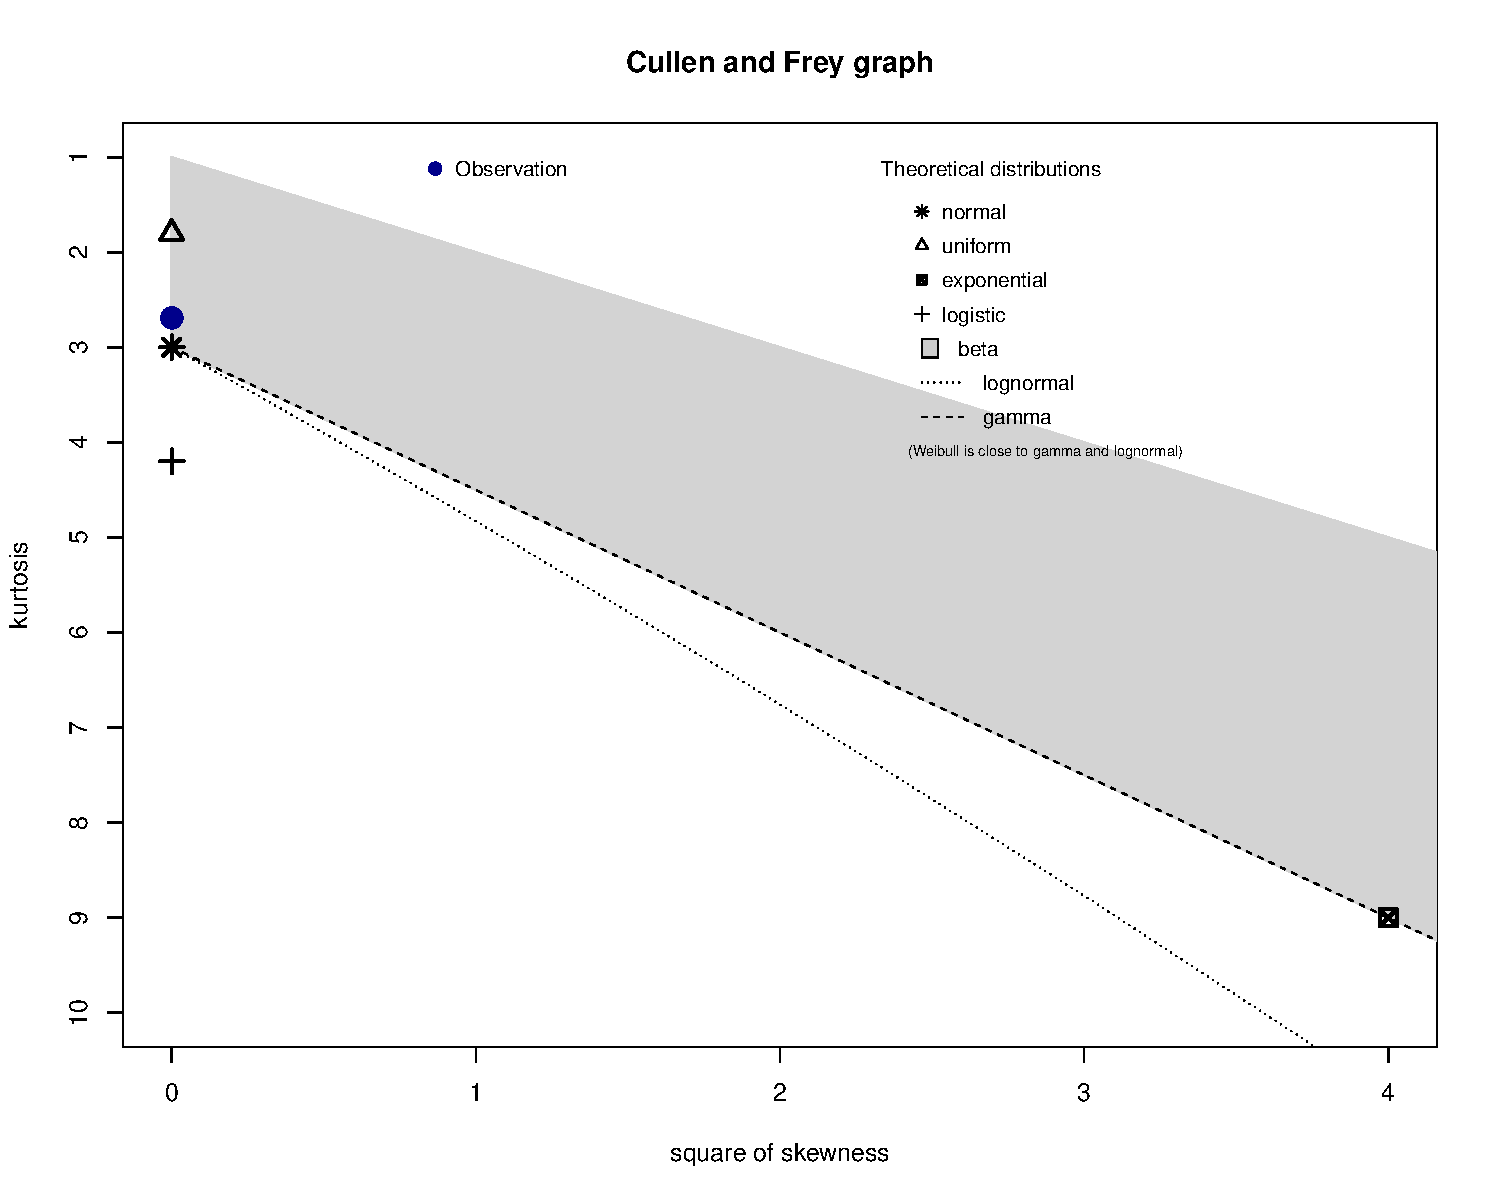
\includegraphics[width=0.85\linewidth]{Images/FIGURES/descdist_density}
	\caption{Diagram šikmost-strmost vzhledem k různým distribucím pro hustotu těla mužů.}
	\label{fig:descdist_density}
\end{figure}

\begin{figure}[ht!]
	\centering
	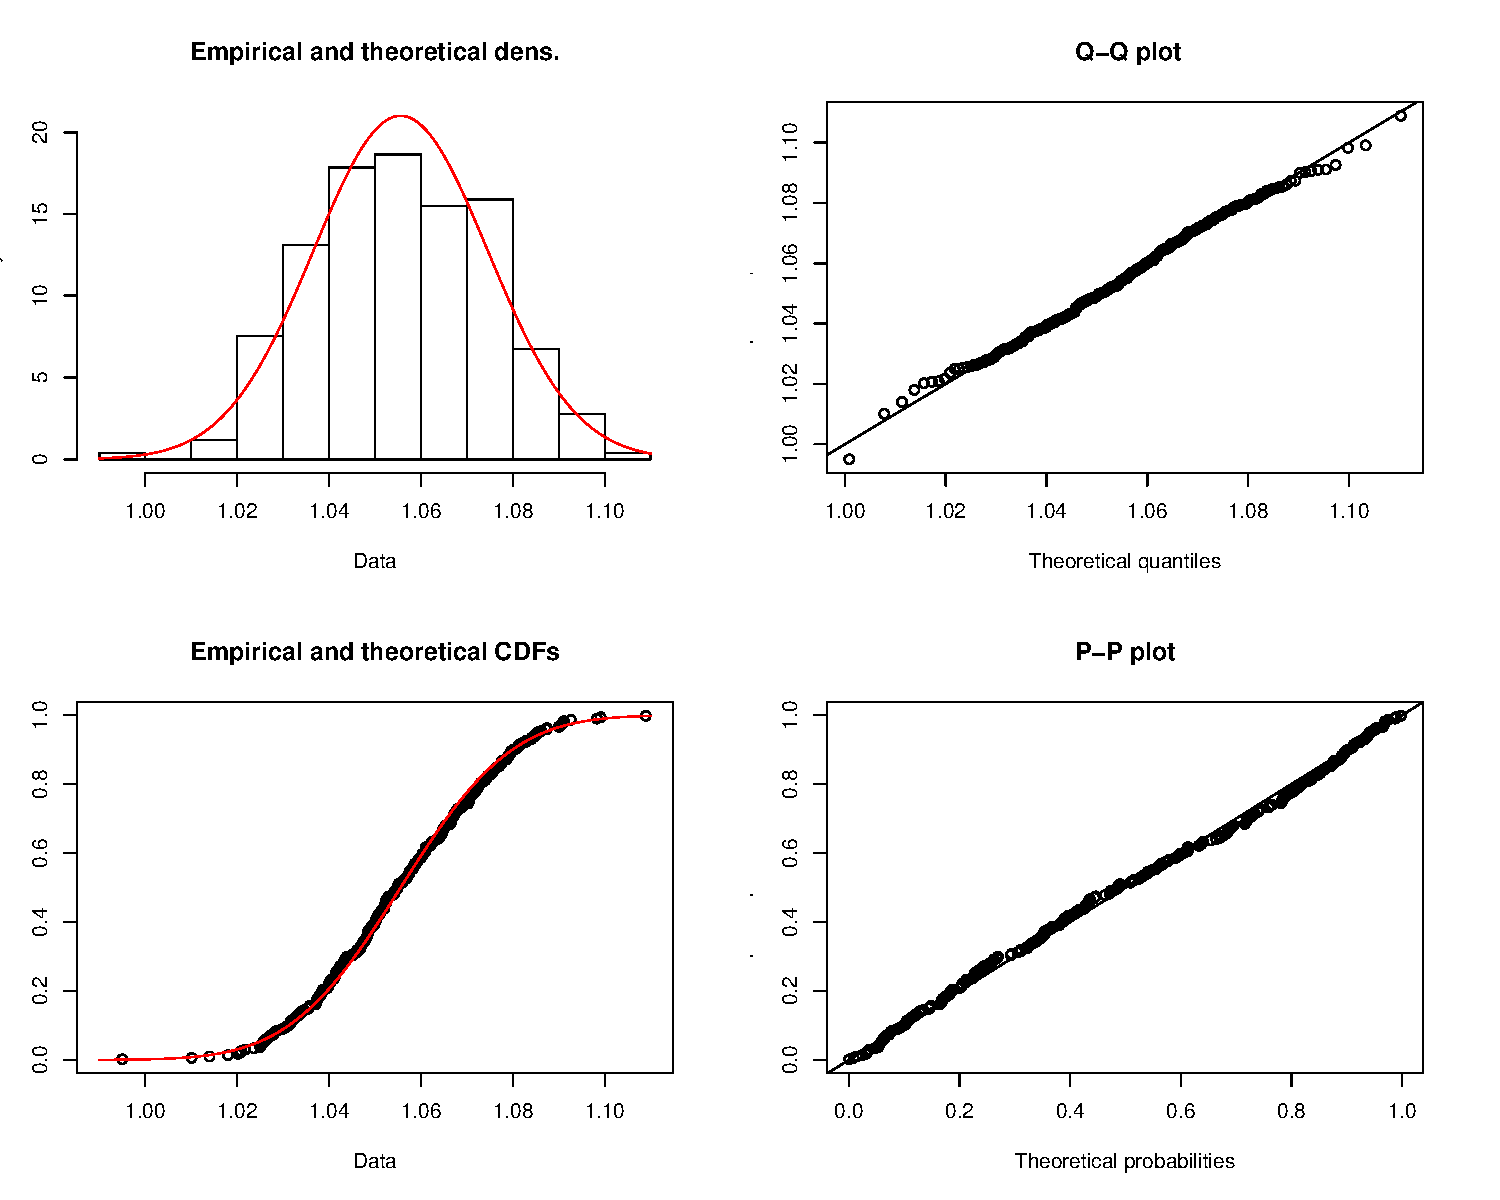
\includegraphics[width=1.0\linewidth]{Images/FIGURES/density_fitdist}
	\caption{Fit normálního rozdělení pro hustotu těla mužů.}
	\label{fig:density_fitdist}
\end{figure}

\newpage

%\newpage{}
%
%\bibliography{bib/Benes2017,bib/MMC}
%
%%\bibliographystyle{plain}
%\bibliographystyle{alpha}

\end{document}
